\documentclass[portrait,a0paper,fontscale=0.277]{baposter}

\usepackage{calc}
\usepackage{graphicx}
\usepackage{amsmath}
\usepackage{amssymb}
\usepackage{relsize}
\usepackage{multirow}
\usepackage{rotating}
\usepackage{bm}
\usepackage{url}

%\usepackage{graphicx}
\usepackage{multicol}

%\usepackage{times}
%\usepackage{helvet}
%\usepackage{bookman}
\usepackage{palatino}

\newcommand{\captionfont}{\footnotesize}

\graphicspath{{images/}{../images/}}
\usepackage{tikz}                                                                                                                                                                                    
\usetikzlibrary{arrows,shapes,calc}

\newcommand{\SET}[1]  {\ensuremath{\mathcal{#1}}}
\newcommand{\MAT}[1]  {\ensuremath{\boldsymbol{#1}}}
\newcommand{\VEC}[1]  {\ensuremath{\boldsymbol{#1}}}
\newcommand{\Video}{\SET{V}}
\newcommand{\video}{\VEC{f}}
\newcommand{\track}{x}
\newcommand{\Track}{\SET T}
\newcommand{\LMs}{\SET L}
\newcommand{\lm}{l}
\newcommand{\PosE}{\SET P}
\newcommand{\posE}{\VEC p}
\newcommand{\negE}{\VEC n}
\newcommand{\NegE}{\SET N}
\newcommand{\Occluded}{\SET O}
\newcommand{\occluded}{o}

%%%%%%%%%%%%%%%%%%%%%%%%%%%%%%%%%%%%%%%%%%%%%%%%%%%%%%%%%%%%%%%%%%%%%%%%%%%%%%%%
%%%% Some math symbols used in the text
%%%%%%%%%%%%%%%%%%%%%%%%%%%%%%%%%%%%%%%%%%%%%%%%%%%%%%%%%%%%%%%%%%%%%%%%%%%%%%%%

%%%%%%%%%%%%%%%%%%%%%%%%%%%%%%%%%%%%%%%%%%%%%%%%%%%%%%%%%%%%%%%%%%%%%%%%%%%%%%%%
% Multicol Settings
%%%%%%%%%%%%%%%%%%%%%%%%%%%%%%%%%%%%%%%%%%%%%%%%%%%%%%%%%%%%%%%%%%%%%%%%%%%%%%%%
\setlength{\columnsep}{1.5em}
\setlength{\columnseprule}{0mm}

%%%%%%%%%%%%%%%%%%%%%%%%%%%%%%%%%%%%%%%%%%%%%%%%%%%%%%%%%%%%%%%%%%%%%%%%%%%%%%%%
% Save space in lists. Use this after the opening of the list
%%%%%%%%%%%%%%%%%%%%%%%%%%%%%%%%%%%%%%%%%%%%%%%%%%%%%%%%%%%%%%%%%%%%%%%%%%%%%%%%
\newcommand{\compresslist}{%
\setlength{\itemsep}{1pt}%
\setlength{\parskip}{0pt}%
\setlength{\parsep}{0pt}%
}

%%%%%%%%%%%%%%%%%%%%%%%%%%%%%%%%%%%%%%%%%%%%%%%%%%%%%%%%%%%%%%%%%%%%%%%%%%%%%%
%%% Begin of Document
%%%%%%%%%%%%%%%%%%%%%%%%%%%%%%%%%%%%%%%%%%%%%%%%%%%%%%%%%%%%%%%%%%%%%%%%%%%%%%

\begin{document}
\typeout{Poster Starts}
\background{
\begin{tikzpicture}[remember picture,overlay]%
\draw (current page.north west)+(-2.62em,2.4em) node[anchor=north west] {
\includegraphics[height=1.\textheight]{PDFTemplate}};
\end{tikzpicture}%
}

%%%%%%%%%%%%%%%%%%%%%%%%%%%%%%%%%%%%%%%%%%%%%%%%%%%%%%%%%%%%%%%%%%%%%%%%%%%%%%
%%% Here starts the poster
%%%---------------------------------------------------------------------------
%%% Format it to your taste with the options
%%%%%%%%%%%%%%%%%%%%%%%%%%%%%%%%%%%%%%%%%%%%%%%%%%%%%%%%%%%%%%%%%%%%%%%%%%%%%%
% Define some colors

%\definecolor{lightblue}{cmyk}{0.83,0.24,0,0.12}
\definecolor{lightblue}{rgb}{0.2667,0.2706,0.4627}
\definecolor{darkblue}{rgb}{0.5490,0.2039,0.8353}
\definecolor{lightpurple}{rgb}{0.8,0.8,1}

\definecolor{silver}{cmyk}{0,0,0,0.3}
\definecolor{yellow}{cmyk}{0,0,0.9,0.0}
\definecolor{reddishyellow}{cmyk}{0,0.22,1.0,0.0}
\definecolor{black}{cmyk}{0,0,0.0,1.0}
\definecolor{darkYellow}{cmyk}{0,0,1.0,0.5}
\definecolor{darkSilver}{cmyk}{0,0,0,0.1}
\definecolor{lightyellow}{cmyk}{0,0,0.3,0.0}
\definecolor{lighteryellow}{cmyk}{0,0,0.1,0.0}
\definecolor{lightestyellow}{cmyk}{0,0,0.05,0.0}
\definecolor{thalesMarine}{cmyk}{0.95,0.90,0,0.3}
\definecolor{thalesTurquoise}{cmyk}{0.76,0,0.1,0}
%\definecolor{midnightblue}{cmyk}{1,1,0,0.5}
\definecolor{midnightblue}{cmyk}{0.78,0.78,0,0.56}
\definecolor{bloodred}{cmyk}{0,1,1,0.6}
\definecolor{lavender}{cmyk}{0.08,0.08,0,0.02}
\definecolor{pine}{cmyk}{0.18,0.0,0.77,0.69}
\definecolor{olive}{cmyk}{0.24,0.0,0.76,0.45}
\definecolor{pinegreen}{cmyk}{1.0,0.0,1.0,1.0}
\definecolor{clover}{cmyk}{0.61,0.0,0.47,0.37}
\definecolor{indianred}{cmyk}{0.0,0.58,0.58,0.0}
\definecolor{mistyrose}{cmyk}{0.0,0.31,0.32,0.6}
%\definecolor{mistyrose}{cmyk}{0.0,0.11,0.12,0.2}
\definecolor{deeppurple}{cmyk}{0.0,0.81,0.4,0.67}

 
% Draw a video
%% \newlength{\FSZ}
%% \newcommand{\drawvideo}[3]{% [0 0.25 0.5 0.75 1 1.25 1.5]
%%    \noindent\pgfmathsetlength{\FSZ}{\linewidth/#2}
%%    \begin{tikzpicture}[outer sep=0pt,inner sep=0pt,x=\FSZ,y=\FSZ]
%%    \draw[color=lightblue!50!black] (0,0) node[outer sep=0pt,inner sep=0pt,text width=\linewidth,minimum height=0] (video) {\noindent#3};
%%    \path [fill=lightblue!50!black,line width=0pt] 
%%      (video.north west) rectangle ([yshift=\FSZ] video.north east) 
%%     \foreach \x in {1,2,...,#2} {
%%       {[rounded corners=0.6] ($(video.north west)+(-0.7,0.8)+(\x,0)$) rectangle +(0.4,-0.6)}
%%     }
%% ;
%%    \path [fill=lightblue!50!black,line width=0pt] 
%%      ([yshift=-1\FSZ] video.south west) rectangle (video.south east) 
%%     \foreach \x in {1,2,...,#2} {
%%       {[rounded corners=0.6] ($(video.south west)+(-0.7,-0.2)+(\x,0)$) rectangle +(0.4,-0.6)}
%%     }
%% ;
%%    \foreach \x in {1,...,#1} {
%%      \draw[color=lightblue!50!black] ([xshift=\x\linewidth/#1] video.north west) -- ([xshift=\x\linewidth/#1] video.south west);
%%    }
%%    \foreach \x in {0,#1} {
%%      \draw[color=lightblue!50!black] ([xshift=\x\linewidth/#1,yshift=1\FSZ] video.north west) -- ([xshift=\x\linewidth/#1,yshift=-1\FSZ] video.south west);
%%    }
%%    \end{tikzpicture}
%% }

\hyphenation{resolution occlusions}
%%
\begin{poster}%
  % Poster Options
  {
  % Show grid to help with alignment
  grid=false,
  % Column spacing
  colspacing=1em,
  % Color style
	%bgColorOne=lighteryellow,
  %bgColorTwo=lightestyellow,
bgColorOne=white,
  %bgColorTwo=white,
%bgColorTwo=lightpurple,
%bgColorTwo=darkSilver,
bgColorTwo=lavender,
%bgColorTwo=reddishyellow,
	%bgColorTwo=silver,
  borderColor=mistyrose,
  headerColorOne=pine,
  headerColorTwo=olive,
  headerFontColor=white,
  boxColorOne=white,
  boxColorTwo=lightblue,
  % Format of textbox
  textborder=roundedleft,
  % Format of text header
  eyecatcher=true,
	%eyecatcher=false,
  headerborder=closed,
  headerheight=0.1\textheight,
%  textfont=\sc, An example of changing the text font
  headershape=roundedright,
  headershade=shadelr,	
	%headerfont=\Large\bf\textsc, %Sans Serif
	headerfont=\Large\bf, %Sans Serif
%  textfont={\color{deeppurple}\setlength{\parindent}{0em}},
  textfont={\color{pinegreen}\setlength{\parindent}{0em}},
%  textfont={\setlength{\parindent}{1.5em}},
%headerFontColor=thalesMarine,
  %boxshade=plain,
	boxshade=none,
  %background=none,
  %background=shadetb,
  %background=plain,
	background=user,
  linewidth=2pt
  }
  % Eye Catcher
	{
	\makebox[10em]{ }
	}
	%{
\includegraphics[scale=0.3]{PDFTemplate}}
  %{\includegraphics[scale=0.3]{logo_gecco2013}}
  %{\includegraphics[height=5em]{logo_lri}}
  % Title
{\color{purple} Pareto-Based Multiobjective\\ AI Planning\vspace{0.3em}}
  % Authors
%{\color{bloodred} \large Mostepha-Redouane Khouadjia, Marc Schoenauer, Vincent Vidal, Johann Dr\'eo, Pierre Sav\'eant}
{ \color{bloodred} M.R. Khouadjia, M. Schoenauer, V. Vidal, J. Dr\'eo, P. Sav\'eant}
  %{\bf\textsc{Multiobjective Optimization for Reducing Delays and Congestion in ATM}}
  % Authors
  %{{\large \textsc{\{gaetan.marceaucaron, pierre.saveant\}@thalesgroup.com \\ marc.schoenauer@inria.fr}}}
  % University logo
{% The makebox allows the title to flow into the logo, this is a hack because of the L shaped logo.

\begin{tabular}[]{r}
%\includegraphics[scale=0.12]{logo_lri}\\

\includegraphics[scale=0.4]{thales_q}\\
%\includegraphics[scale=0.14]{cnrsfilaire_quadri} \hspace{0.3cm}
%\includegraphics[scale=0.25]{logoCNRS} \hspace{0.3cm}

\includegraphics[scale=0.15]{ONERA_logo}\\

\includegraphics[scale=0.2]{logo_inria}
\end{tabular}

%\makebox[8em][r]{%
%\begin{minipage}{16em}
%\hfill
%\includegraphics[scale=0.1]{logo-lri}\\
%
\includegraphics[scale=0.1]{hd_logo_thales}\\
%\includegraphics[scale=0.05]{INRIA_CORPO_UK_CMJN}
%\end{minipage}
}


%%%%%%%%%%%%%%%%%%%%%%%%%%%%%%%%%%%%%%%%%%%%%%%%%%%%%%%%%%%%%%%%%%%%%%%%%%%%%%
%%% Now define the boxes that make up the poster
%%%---------------------------------------------------------------------------
%%% Each box has a name and can be placed absolutely or relatively.
%%% The only inconvenience is that you can only specify a relative position 
%%% towards an already declared box. So if you have a box attached to the 
%%% bottom, one to the top and a third one which should be in between, you 
%%% have to specify the top and bottom boxes before you specify the middle 
%%% box.
%%%%%%%%%%%%%%%%%%%%%%%%%%%%%%%%%%%%%%%%%%%%%%%%%%%%%%%%%%%%%%%%%%%%%%%%%%%%%%
    %
    % A coloured circle useful as a bullet with an adjustably strong filling
\newcommand{\colouredcircle}{%
\tikz{\useasboundingbox (-0.2em,-0.32em) rectangle(0.2em,0.32em); \draw[draw=black,fill=lightblue,line width=0.03em] (0,0) circle(0.18em);}}

\headerbox{Motivation}{name=problem,column=0,row=0}{
xxxxxxxxxxxxxxxxxxxxx :
\begin{enumerate}\compresslist
\item A
\item B
\item C
\item D
\end{enumerate}
XXXXXXXXXX

XXXXXXXXXX

XXXXXXXXXX

XXXXXXXXXX

XXXXXXXXXX

XXXXXXXXXX


\vspace{0.3em}
}
    
\headerbox{Multiobjective Evolutionary Algorithms}{name=method,column=0,below=problem}{
XXXXXXXXXXX

XXXXXXXXXX

XXXXXXXXXX

XXXXXXXXXX

XXXXXXXXXX


\vspace{0.3em}
}
    
\headerbox{Multiobjective Divide-and-Evolve}{name=flight_model,column=1,span=2,row=0}{
XXXXXXXXXX

XXXXXXXXXX

XXXXXXXXXX

XXXXXXXXXX

XXXXXXXXXX

XXXXXXXXXX

XXXXXXXXXX

XXXXXXXXXX

XXXXXXXXXX

XXXXXXXXXX

XXXXXXXXXX

XXXXXXXXXX

\vspace{0.3em}
}

\headerbox{Benchmark Domains and Instances}{name=sector_model,column=1,span=2,below=flight_model}{
XXXXXXXXXX

XXXXXXXXXX

XXXXXXXXXX

XXXXXXXXXX

XXXXXXXXXX

XXXXXXXXXX

XXXXXXXXXX

XXXXXXXXXX

XXXXXXXXXX

\vspace{0.3em}
}

\headerbox{Results}{name=optimization,column=1,span=2,below=sector_model}{
XXXXXXXXXX

XXXXXXXXXX

XXXXXXXXXX

XXXXXXXXXX

XXXXXXXXXX

XXXXXXXXXX

XXXXXXXXXX

XXXXXXXXXX
\begin{center}
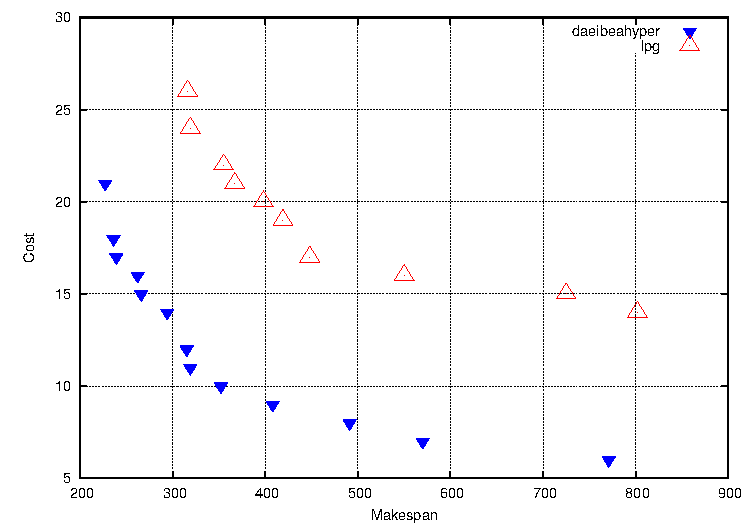
\includegraphics[scale=0.5]{p05_openstacks_Add_dae_pareto}  \hspace{1cm} 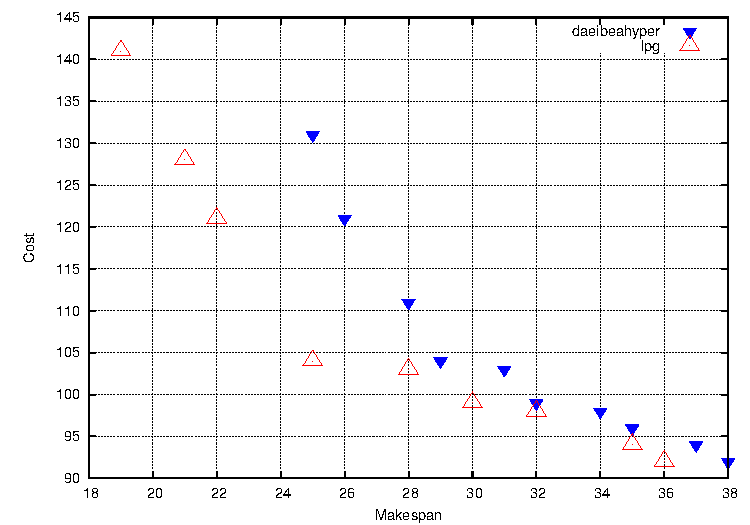
\includegraphics[scale=0.5]{pfile3_floortile_Add_dae_pareto}\\
\hspace{-3.cm} Openstacks5 \hspace{5.3cm} Floortile03 
\end{center}



\vspace{0.3em}
}
		
\headerbox{Acknowledgement}{name=source,column=2,below=optimization,above=bottom}{This work was partially funded by the DESCARWIN ANR project (ANR-09-COSI-002)}
    
\headerbox{Conclusion}{name=further_research,column=1,span=1,below=optimization,above=bottom}{
XXXXXXXXXX

XXXXXXXXXX

XXXXXXXXXX

XXXXXXXXXX
\vspace{0.3em}
}
		
		
\headerbox{Divide-and-Evolve}{name=queries,column=0,below=method}{
XXXXXXXXXX

XXXXXXXXXX

XXXXXXXXXX

XXXXXXXXXX
\vspace{0.3em}
}

	
\headerbox{Experiments}{name=references,column=0,,below=queries,above=bottom}{

    }

\end{poster}

\end{document}

